%
%RESULTS Rev1: Notebook Rev1_15 bevat de exacte cijfers.

\begin{figure*}[htbp!]
	\centering
	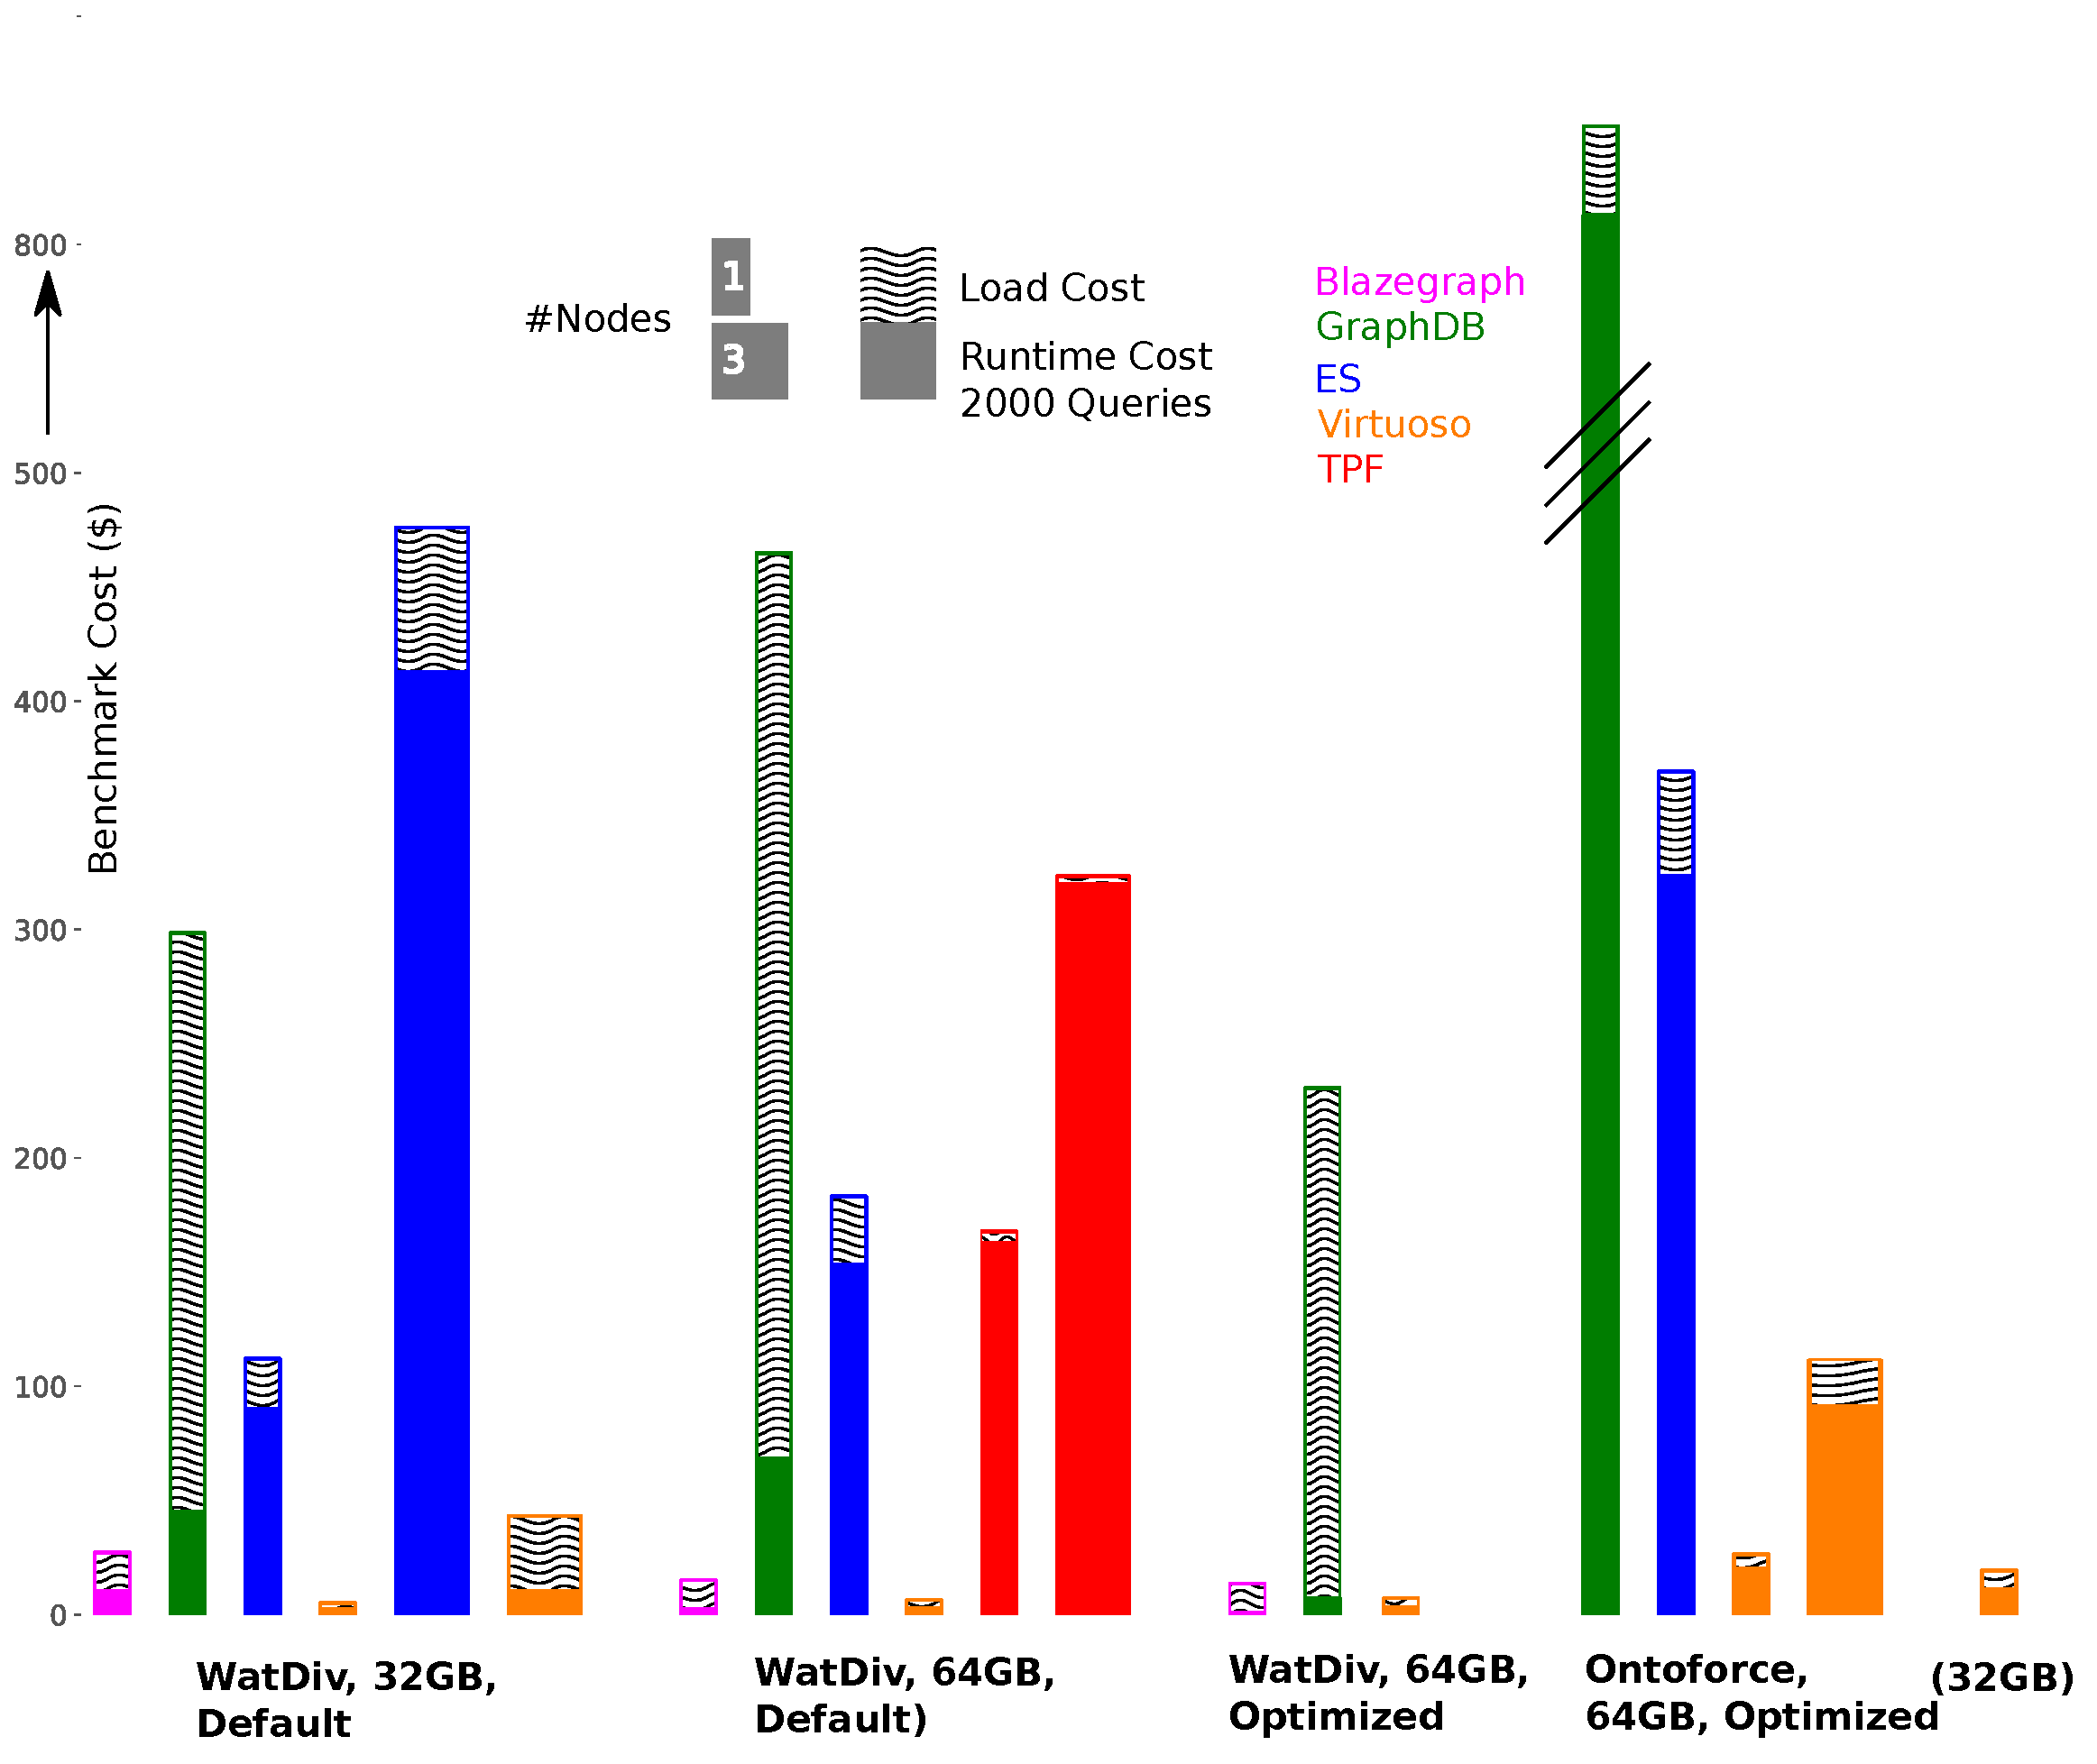
\includegraphics[width=0.9\linewidth]{imgs/Fig11_AllSims_Correct}
	\caption{Benchmark Cost in \$ to load and execute 2000 queries in a stress test for WatDiv1000M or Ontoforce datasets for different setups. All stacked bars consists the load cost stacked on top of the runtime cost. Bar width encodes the amount of nodes. For WatDiv \textbf{Vir1\_32\_Def} is the least expensive solution, mainly because \textbf{Bla1\_64\_Opt} has a much higher load cost. Also for the Ontoforce benchmark\textbf{ Vir1\_32\_Opt} is the most cost-effective choice. The engine ranking is not conserved going from artificial to real-world benchmark.}
	\label{fig:Fig11_AllSims_Correct}
\end{figure*}

In this section we aim to get a satellite view on the entire set of benchmarks conducted within this research. The penultimate trade-off for many applications in production is the cost for processing a certain workload. Our choice for using cloud hardware and AMIs enables this integrated view on all benchmarks: using cost we can compare single to multi-node setups, the cost for vertical scaling,... 

All costs per store and for all benchmarks are shown in Figure~\ref{fig:Fig11_AllSims_Correct}. 
Costs stem from an hourly price for servers on Amazon EC2, together with an hourly license cost for the AMIs.

The instance cost of the AWS hardware was \\ \mbox{\$0.333 /hr} for the 32GB server instances and \\\$0.667 /hr for the 64GB instances. The licensing costs for the PAGO instances can be found on AWS marketplace and typically scale with the amount of memory per instance. For the 64GB instances, GraphDB's license cost is \$1.4 /hr, for ES \$2 /hr and for Virtuoso \$0.80 /hr. Other systems tested have no licensing cost.

Additionally, before running a benchmark the data has to be ingested in the system. This cost is stacked on top of the query cost in Figure~\ref{fig:Fig11_AllSims_Correct}. For some cases the ingest cost is unimportant as reloading the data is required only rarely.

\begin{itemize}
	\item \textbf{The price of vertical scaling:} Is adding more memory, and therefore a higher license and infrastructure cost a wise choice? If we focus on the \emph{Optimized} configurations for Watdiv1000M both \textbf{Bla1} and \textbf{Gra1} have lower operational costs when running the higher end hardware. For \textbf{Bla1} the price is lowered from \$27 to \$13.5, for \textbf{Gra1} the reduction is from \$298 to \$230. For the latter mainly the bulk loading process makes it less competitive. For \textbf{Vir1} the price goes from \$5 to \$7.
	
	%LsF 168-> 323 => x2
	%Es  112 -> 475 => x4
	%Vir 5 -> 42
	\item \textbf{The price of horizontal scaling:} As adding more nodes led to higher runtimes, this also translates to higher costs. For \textbf{TPF} the costs go from \$168 to \$323 ($\times 1.9$) , for \textbf{ES} the costs rises from \$112 to \$475 ($\times 4.2$) and for \textbf{Vir} from \$5 to \$42 ($\times 8.4$) 

	\item \textbf{The price for data ingestion:} \textbf{Gra1} seems to have the highest cost for loading the datasets, except for the Ontoforce benchmark. This is interesting as the Ontoforce benchmark has a much bigger dataset (2.4 BT). A possible explanation is that \textbf{Gra1} has trouble ingesting a single gzipped turtle file as was the case for WatDiv, while the Ontoforce dataset was ingested as 42 gzipped N-Quads files.
    For \textbf{Gra1\_64\_Def} many additional indexes are generated during ingest, which explains the lower cost for \textbf{Gra1\_64\_Opt}. Having more memory by itself can also impact the ingest process, for \textbf{Bla1} the ingest cost is lowered from \$16 to \$12. Virtuoso's bulk loader process is a real trump 
    card in the cost comparisons. The load cost is \$2.8 while \textbf{Bla1} in the optimal case has a cost of \$12.6. The load cast is in fact larger than the runtime cost in this comparison.
    Also for the multi-node setups no advantage is obtained in the ingest phase. \textbf{Vir3} takes 4 times more time to ingest while the cost/hr is also 3 times higher. For \textbf{ES3} a 33\% cost increase is measured, while for \textbf{TPF3} the ingestion becomes 50\% cheaper. The latter however is not \textbf{TPF} specific as the ingestion corresponds to the partitioning and compression of the data with the HDT algorithm.

	\item \textbf{The most cost-effective solution:} \textbf{Vir1\_32} is the cheapest solution both for WatDiv1000M as for the Ontoforce benchmark, with costs of respectively \$5 and  \$19. 
\end{itemize}
%SiM						%run2000_cost	load_cost	
%
%Bla_N1_32_W1000_Def		10.440997		16.775985
%Es_N1_32_W1000_Def			90.264271		21.813804
%Gra_N1_32_W1000_Def		45.081634		253.422000
%Vir_N1_32_W1000_Def		2.267796		2.811233
%
%Es_N3_32_W1000_Def			412.789135		63.223079
%Vir_N3_32_W1000_Def		10.366335		32.821250
%
%Bla_N1_64_W1000_Def		2.490707		12.625764
%Es_N1_64_W1000_Def			153.441334		29.685139
%Gra_N1_64_W1000_Def		68.333470		396.480000
%Vir_N1_64_W1000_Def		2.974605		3.411128
%
%Bla_N1_64_W1000_Opt		0.718728		12.862393
%Gra_N1_64_W1000_Opt		7.251239		223.295333
%Vir_N1_64_W1000_Opt		3.288285		3.754633
%
%LdF_N1_64_W1000_Def		162.507679		5.087619
%LdF_N3_64_W1000_Def		319.976409		3.372289
%
%Es_N1_64_Ont_Def			323.740838		45.506300
%Gra_N1_64_Ont_Opt			813.048618		38.892554
%Vir_N1_32_Ont_Opt_VWall	11.172173		8.161853
%Vir_N1_64_Ont_Opt			20.400952		6.107667
%Vir_N3_64_Ont_Opt_0		91.448916		20.090817
 